%\part{Aplicaciones.}
\chapter{Aplicaciones}
\label{chap:8}
\lhead{Cap\'itulo 7. \emph{Aplicaciones}}

\epigraph{ \textit{`` SUSY is a wonderful woman who does not return my letters. It makes you wonder if she even exists! "} }{ Csaba Csaki~\cite{FrancisOnCsakaWeb2012}}

Uno de los objetivos de este capítulo es el de  poner a prueba el formalismo para el caso más sencillo, la interacción cúbica  de un  supercampo escalar. Para este caso, tenemos la contraparte canónica bien establecida: El modelo de Wess-Zumino. Toca demostrar la equivalencia entre este modelo y nuestro enfoque nocanónico. 
   
  % Damos un paso adelante y proponemos un nuevo modelo canónico para la superparticula de superespin $ 1/2 $ usando supercampos de Dirac. Como demostraremos, la característica particular de estos supercampos es que en el esquema de interacción satisfacen todos los criterios de los supercampos encontrados con los métodos nocanónicos. Ademas los propagadores, encontrados  con ambos métodos, coinciden. Por otro lado, usamos las directrices que nos a dejado el formalismo, para ir en busca de
\section{El Supercampo Escalar}\label{Sec_ScalarSuperPotential}
%Esta sección tiene como objetivo poner a prueba el formalismo para el caso más sencillo: El supercampo escalar. Consideramos a detalle el potencial cubico, esto es, el modelo de Wess-Zumino.

Para el caso escalar, las transformaciones $ C $, $ P $,  $ T$ and $ \mathcal{R} $ se ven como 
      \begin{IEEEeqnarray}{rl}
            \mathsf{C}\,\Phi_{\pm }\left( x,\vartheta\right) \mathsf{C}^{-1}   & \, = \, +{\varsigma}^{\,*} {\Phi}^{\dagger}_{\pm }\left( x,\vartheta\right) \  \nonumber \\
                \mathsf{P} \,\Phi_{\pm}\left( x,\vartheta\right)   \mathsf{P}^{-1}    &\, = \, \pm{\eta}^{*}\,{\Phi}_{\mp}\left(\mathcal{P} x,i\beta\vartheta\right) \ , \nonumber\\
                            \mathsf{T} \,\Phi_{\pm}\left( x,\vartheta\right)   \mathsf{T}^{-1}     & \, = \, \pm {\xi}^{*} \Phi_{\pm  }\left(\mathcal{T} x,\epsilon\gamma_{5}\vartheta^{*}\right) \ , \nonumber \\
                             \mathsf{R}\,\Phi_{\pm }\left( x,\vartheta\right) \mathsf{R}^{-1}    & \, = \, +{r}^{*}\,\Phi_{\pm }\left( x,D_{\mathcal{R}}\vartheta\right)  \ . \nonumber \\
    \label{8-01-01}
\end{IEEEeqnarray}
Cuando la spartícula es la misma que su antispartícula, 
\begin{IEEEeqnarray}{rl}
         \Phi_{\pm}(x,\vartheta) & \, = \,  \Phi^{\dagger}_{\pm}(x,\vartheta)  \ ,   
    \label{8-01-02}
\end{IEEEeqnarray}     
además,  $ \varsigma $, $ \eta $, $ \zeta $ y $ r $ son  iguales a $ \pm 1 $.  La interacción de orden m\'as bajo, el superpotencial cúbico, posee cuatro términos:
\begin{IEEEeqnarray}{rl}
            \Phi_{\pm}\Phi_{\pm}\Phi_{\pm}, \quad \Phi_{\pm}\Phi_{\pm}\Phi^{\dagger}_{\pm}, \quad\Phi_{\pm}\Phi^{\dagger}_{\pm}\Phi^{\dagger}_{\pm},\quad \Phi^{\dagger}_{\pm}\Phi^{\dagger}_{\pm}\Phi^{\dagger}_{\pm} \ .
    \label{8-01-03}
\end{IEEEeqnarray}
  Bajo una transformación  $ \mathcal{R} $, usando el hecho de que
\begin{IEEEeqnarray}{rl}
                \delta^{2}\left( \mathcal{R}^{-1}\vartheta_{\pm} \right)  \, = \, \exp\left[ \pm 2i q_{0} \right]\delta^{2}\left(\vartheta_{\pm} \right)   \ ,
    \label{08-01-03-01}
\end{IEEEeqnarray}
 estos términos generan las siguientes fases en el superpotencial:
\begin{IEEEeqnarray}{rl}
            -3q\pm q_{0}, \quad -q\pm q_{0},\quad  +q\pm q_{0}, \quad 3q\pm q_{0} \ .
    \label{8-01-04}
\end{IEEEeqnarray}
Entonces, para superpotenciales cúbicos que son $ \mathcal{R} $-simétricos, solo uno de ellos (de los cuatro posibles) sobrevive. Para una spartícula que es su propia antispartícula \eqref{8-01-02}, las cuatro posibilidades \eqref{8-01-03} se vuelven una.
Para ver en acción el formalismo, consideremos el siguiente superpotencial cúbico
\begin{IEEEeqnarray}{rl}
             \mathcal{W}_{+}\left( x, \vartheta \right)   \, = \,  \frac{g_{+}}{3!}  \left( \Phi_{+}\left( x, \vartheta \right)\right)  ^{3}  \, + \, \frac{ g^{*}_{-}}{3!} \left( \Phi^{\dagger}_{+}\left( x, \vartheta \right) \right) ^{3}\ ,  \nonumber \\
              \mathcal{W}^{\dagger}_{-}\left( x, \vartheta \right)   \, = \,  \frac{g_{-}}{3!} \left( \Phi_{-}\left( x, \vartheta \right)\right)  ^{3}  \, + \, \frac{g^{*}_{+}}{3!} \left( \Phi^{\dagger}_{-}\left( x, \vartheta \right) \right) ^{3}  \ .
     \label{8-01-05}
 \end{IEEEeqnarray} 
Restringiéndonos más aun para los casos cuando $ g_{+} =0 $ o $ g_{-}=0 $, calculamos la superamplitud de un proceso spartícula-antispartícula. A orden más bajo, tenemos solo un superdiagrama para este proceso (Figura \ref{Figure 1}). Para las patas externas,  escogemos las siguientes proyecciones derechas e izquierdas para los cuatro espinores fermiónicos [ver la regla de super Feynman para las superpatas externas, Ecs. \eqref{6-4-04}-\eqref{6-4-11}]:
\begin{figure}[h!]
\begin{center}
    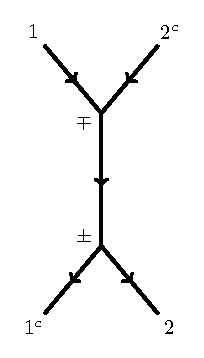
\includegraphics{Figures/Figure_1}
    \caption{ Superdiagrama de menor orden en una colisión spartícula-antispartícula.}
 \label{Figure 1}
 \end{center}
\end{figure}
\begin{IEEEeqnarray}{rl}
            1\rightarrow\pm, \quad 1^{c}\rightarrow\mp,  \quad 2\rightarrow\mp, \quad 2^{c}\rightarrow\pm \ .
    \label{8-01-06}
\end{IEEEeqnarray}
Los signos de arriba(abajo) corresponden a los casos $ g_{-} = 0$($ g_{+} = 0$). La función de onda en el espacio de momentos en el caso del supercampo escalar, es simplemente [ver las Ecs. \eqref{5-3-29} and \eqref{5-3-29}]: 
\begin{IEEEeqnarray}{rl}
            u\left(\mathbf{p} \right)   \, = \,    v\left(\mathbf{p} \right)    \, = \,\frac{1}{\sqrt{2p^{0}}},\quad p^{0} \, = \, \sqrt{\mathbf{p}^{2}  \, + \, m^{2}} \ .
    \label{8-01-07}
\end{IEEEeqnarray}
La contribución de las patas externas al superdiagrama  es 
\begin{IEEEeqnarray}{rl}
     (2\pi)^{-6}\, u(\textbf{p}_{_{2}}) u(\textbf{p}^{c}_{_{1}}) u(\textbf{p}^{c}_{_{2}}) u(\textbf{p}_{_{1}})\,  \times \,       e^{+i x_{_{1}}\cdot\left(  p_{_{1}} -p^{c}_{_{2}}  \right) }   \,   e^{+i x_{_{2}}\cdot \left( p^{c}_{_{1}}  \, - \, p_{_{2}}\right)   }  \nonumber \\
    \times \,\, e^{ 2\left[ {s}_{_{1}}\cdot(+i\slashed{p}_{_{1}})     \, - \, s_{_{2}}^{c}\cdot\, (+i\slashed{p}^{c}_{_{2}})\, \right]{\vartheta}_{_{1}\mp} }\times        e^{  2\left[ {s}_{_{1}} ^{c} \cdot\, (+i\slashed{p}^{c}_{_{1}}) \, - \,{s}_{_{2}} \cdot \, (+i\slashed{p}_{_{2}})\right] \,\vartheta_{_{2}\pm}}\ . \nonumber \\
    \label{8-01-08}
\end{IEEEeqnarray}
Al escribir las exponenciales fermiónicas  hemos usado el hecho de que el  superpotencial $ \mathcal{W}_{\pm} $ esta evaluado en $ (x,\vartheta_{\pm}) $. La contribución de los vértices y la línea interna es
\begin{IEEEeqnarray}{rl}
           \left( 9\times 4\right)  \times \left[ \left( +i\right)^{2} \left( -i\right)^{2}  \left(3! \right)^{-2}  \vert g_{\pm}\vert^{2}\right] \times \left[  \left(-i\right) \left(2\pi \right)^{-4}  \int d^{4}q   \frac{ e^{i\left( x_{_{1}}-x_{_{2}}\right)  \cdot q \, - \, 2\vartheta_{_{1}}^{\intercal}\epsilon\gamma_{5}i\slashed{q}\vartheta_{_{2}\pm}}}{m^{2}+q^{2}-i\varepsilon}\right] \ . \nonumber \\
    \label{8-01-09}
\end{IEEEeqnarray} 
El factor  $ \left( 9\times 4\right)  $,  surge de las posibles combinaciones de formar las lineas internas y externas. Para obtener la superamplitud debemos integrar con 
\begin{IEEEeqnarray}{rl}
            \int d^{4}x_{_{1}}d^{4}x_{_{2}}\,d^{2}\vartheta_{_{1}\mp}\, d^{2}\vartheta_{_{2}\pm} \ .
    \label{8-01-10}
\end{IEEEeqnarray}
Notamos que las integrales de las variables bosónicas nos dan
\begin{IEEEeqnarray}{rl}
              \int d^{4}x_{_{1}} e^{+i x_{_{1}}\cdot\left(  p_{_{1}} -p^{c}_{_{2}}  \, + \, q  \right) }   & \, = \, \left( 2\pi\right)^{4}\delta^{4}\left(  p_{_{1}} -p^{c}_{_{2}}  \, + \, q  \right) \  , \nonumber \\
               \int d^{4}x_{_{2}}   \,   e^{+i x_{_{2}}\cdot \left( p^{c}_{_{1}}  \, - \, p_{_{2}}  \, - \,q\right)   }    &           \, = \, \left( 2\pi\right)^{4}\delta^{4}\left(  p^{c}_{_{1}} -p_{_{2}}  \, - \, q  \right)\ .
    \label{8-01-11}
\end{IEEEeqnarray}
Después de integrar con $ d^{4}q $, obtenemos la expresión siguiente para el superdiagrama \textit{sin} las variables fermiónicas $ \vartheta_{_{1}\mp}$ y  $\vartheta_{_{2}\pm} $ integradas:
\begin{IEEEeqnarray}{rl}
\,\tfrac{1}{4} f_{\text{scalar}} \left( \textbf{p}_{_{1}},\textbf{p}^{c}_{_{1}},\textbf{p}_{_{2}},\textbf{p}^{c}_{_{2}}\right) \, e^{ - 2i {\vartheta}_{{1}\mp}\cdot\left(\slashed{p}_{{1}} {s}_{{1}}   \, - \, \, \slashed{p}^{c}_{2}s_{2}^{c}\, \right)  }      e^{ - 2i\vartheta_{_{2}\pm}\cdot\left(  \, \slashed{p}^{c}_{1}{s}_{1} ^{c}\, - \,  \slashed{p}_{_{2}}{s}_{2}\right) \,}     e^{ \, - \, 2i \vartheta_{_{1}}\cdot \left( \slashed{p}^{c}_{{1}} - \slashed{p}_{{2}}  \right) \vartheta_{_{2}\pm} } \ , \nonumber \\
    \label{8-01-12}
\end{IEEEeqnarray}
con 
\begin{IEEEeqnarray}{rl}
              f_{\text{scalar}} \left( \textbf{p}_{_{1}},\textbf{p}^{c}_{_{1}},\textbf{p}_{_{2}},\textbf{p}^{c}_{_{2}}\right)  &  \, = \,  \left(-4i\right) \vert g_{\pm}\vert^{2}  (2\pi)^{-2}  \,    \delta^{4}\left(  p_{{1}} \, + \,  p^{c}_{{1}} -p^{c}_{{2}}  -p_{{2}}   \right)           \nonumber \\
            & \qquad \times  u(\textbf{p}_{_{2}}) u(\textbf{p}^{c}_{_{1}}) u(\textbf{p}^{c}_{_{2}}) u(\textbf{p}_{_{1}})\,    \times  \left[ {m^{2}+\left( p^{c}_{{1}} -p_{{2}}  \right) ^{2}-i\varepsilon}\right]^{-1}\ .\nonumber \\
    \label{8-01-13}
\end{IEEEeqnarray}
Esta última cantidad, es la expresión para el mismo diagrama pero en el espacio. 
Aislamos la dependencia en la variable $ (\vartheta_{_{1}\mp}) $  e integramos sobre esta variable:
\begin{IEEEeqnarray}{rl}
 \int d^{2}\vartheta_{_{1}\mp}\, e^{ - 2i {\vartheta}_{{1}\mp}\cdot\left[\slashed{p}_{{1}} {s}_{{1}}   \, - \, \, \slashed{p}^{c}_{{2}}s_{{2}}^{c}\, \, + \,  \left( \slashed{p}^{c}_{{1}} - \slashed{p}_{{2}}  \right)\vartheta_{{2}}\right]}    & \, = \, -4\, \delta^{2}\left[\slashed{p}_{{1}} {s}_{{1}}   \, - \, \, \slashed{p}^{c}_{{2}}s_{{2}}^{c}\, \, + \,  \left( \slashed{p}^{c}_{{1}} - \slashed{p}_{{2}}  \right)\vartheta_{{2}}\right]_{\mp}    \nonumber \\
   \, = \,4\left( {p}^{c}_{{1}} - {p}_{{2}}  \right) ^{2} &\delta^{2}\left[ \left( \slashed{p}^{c}_{{1}} - \slashed{p}_{{2}}  \right)^{-1}\left( \slashed{p}_{{1}} {s}_{{1}}   \, - \, \, \slashed{p}^{c}_{{2}}s_{{2}}^{c}\right)\, \, + \,  \vartheta_{{2}}\right]_{\mp}    \ .   \nonumber \\
    \label{8-01-14}
\end{IEEEeqnarray}
Después de integrar con esta función delta  en la variable $ \vartheta_{_{2}\pm}  $, obtenemos la forma final de la superamplitud para la colisión spartícula-antispartícula:
\begin{IEEEeqnarray}{rl}
S^{\mp}\left( \cdots\right)  \, = \, f_{\text{scalar}}\, \times \, \left( {p}^{c}_{{1}} - {p}_{{2}}  \right) ^{2}\times \exp{\left[-2i \, h^{\mp}\left( \cdots\right) \right]} \ ,  \nonumber \\           
    \label{8-01-15}
\end{IEEEeqnarray}
los puntos $ \left( \cdots\right)  $ denotan al superespacio de momentos $  \left(\textbf{p}_{_{1}},s_{_{1}\pm},\textbf{p}^{c}_{_{1}}, s^{c}_{_{1}\mp},\textbf{p}_{_{2}},s_{_{2}\mp},\textbf{p}^{c}_{_{2}}, s^{c}_{_{2}\pm}\right)  $, mientras que la funciones $ h^{\mp} $ vienen dadas por 
\begin{IEEEeqnarray}{rl}
            h^{\mp}\left( \cdots\right)  \, = \, \frac{1}{\left( {p}^{c}_{{1}}  \, - \,{p}_{{2}}  \right)^{2}}\left( \slashed{p}_{{1}} {s}_{{1}}   \, - \, \, \slashed{p}^{c}_{{2}}s_{{2}}^{c}\right) \cdot \left( \slashed{p}^{c}_{{1}} - \slashed{p}_{{2}}  \right)\left(  \, \slashed{p}^{c}_{1}{s}_{1} ^{c}\, - \,  \slashed{p}_{_{2}}{s}_{2}\right)_{\pm}\ .\nonumber \\
    \label{8-01-16}
\end{IEEEeqnarray} 

 La posibilidad de escoger  tres partículas  y tres antipartículas  para la dispersión partícula-antipartícula  nos da un total de $ 3^{4} $ combinaciones de estados iniciales y finales. Desde luego que muchos  de estos procesos son cero, por ejemplo, todos los procesos que provienen de la expansión impar en las variables fermiónicas en la Ec. \eqref{8-01-16} (esto no es otra cosa que una consecuencia que la conservación de momento angular). Vemos de manera explícita la conveniencia de trabajar en una formulación completamente en el superespacio; la  ecuación \eqref{8-01-16} representa una expresión económica para el conjunto de todos los procesos de estas partículas a segundo orden  en la constante de acoplamiento $ \vert  g_{\pm}\vert $.\\

\section{Equivalencia con el Modelo de Wess-Zumino}\label{Sec_TimeOrderedSuperpropagators}
\label{sec:08-02}
Para establecer una equivalencia entre la formulación nocanónica (aquí desarrollada) y la formulación canónica, escribimos el superpropagador no corregido para el supercampo escalar, como aparece en los superpotenciales quirales  (por ahora, hemos omitido un factor de $ -i $):
\begin{IEEEeqnarray}{rl}
  \delta^{2}(\vartheta_{_{1}\mp})\delta^{2}  (\vartheta_{_{2}\pm}) &\tilde{\Delta}^{\pm \mp}\left( x_{_{1}},\vartheta_{_{1}},x_{_{2}},\vartheta_{_{2}}\right)  \nonumber\\
       \, = \,  \delta^{2} & (\vartheta_{_{1}\mp})\delta^{2}  (\vartheta_{_{2}\pm}) \left[1  \, +\, 2 \vartheta_{_{1}}\cdot(-\slashed{\partial}_{_{1}})\vartheta_{_{2}\mp}  \, - \,4 m^{2}\,\delta^{2}(\vartheta_{_{1}\pm})\delta^{2}  (\vartheta_{_{2}\mp})  \right] \Delta_{F}(x_{_{1}}-x_{_{2}}) \ .\nonumber \\  
    \label{08-02-01}
\end{IEEEeqnarray}
Haciendo uso de $ \left( \square - m^{2}\right)\Delta_{F}(x)  \, = \, -\delta^{4}(x) $, escribimos
\begin{IEEEeqnarray}{ll}
  \delta^{2}(\vartheta_{_{1}\mp})\delta^{2}  (\vartheta_{_{2}\pm}) &\tilde{\Delta}^{\pm \mp}\left( x_{_{1}},\vartheta_{_{1}},x_{_{2}},\vartheta_{_{2}}\right)   \nonumber\\
  &  \, = \,\delta^{2}(\vartheta_{_{1}\mp})\delta^{2}  (\vartheta_{_{2}\pm}) \,  \Delta_{F}\left( x^{\pm}_{_{12}}\right)  \, - \, 4  \,\delta^{4}(\vartheta_{_{1}})\,\delta^{4}  (\vartheta_{_{2}})\delta^{4}(x_{_{1}}-x_{_{2}}) \ .  \nonumber \\
    \label{08-02-02}
\end{IEEEeqnarray}
El término $ \, +\, 4 i\,\delta^{4}(\vartheta_{_{1}})\delta^{4}  (\vartheta_{_{2}})\delta^{4}(x_{_{1}}-x_{_{2}}) $ es invariante de Lorentz pero no invariante supersimétrico. Puesto que esta expresión es local en el superespacio, la parte no-covariante del superpropagador  induce términos no covariantes en las interacciones. En el caso de superpotenciales de supercampos arbitrarios, para darnos una idea de su forma, recordamos que aunque la función paso es invariante de Lorentz (excepto en separaciónes del tipo-espacial, donde para lograr la invariancia de Lorentz los conmutadores deben de hacerse cero) no es invariante supersimétrica.  La función paso $ \omega $ seria invariante supersimétrica, si estuviese evaluada en  $   x^{\pm\,0}_{_{12}} $ o incluso en  $  x^{0}_{_{12}}-\vartheta_{_{1}}\cdot\gamma^{0}\vartheta_{_{2}} $. Tomando en cuenta que las funciones  $ \Delta_{+} $ que aparecen en la Ec. \eqref{08-02-02} están evaluadas en  $   x^{\pm\,0}_{_{12}} $, escribimos 
\begin{IEEEeqnarray}{rl}
              \omega\left( x^{0}_{_{12}}\right) \, = \,  \omega\left(  x^{\pm\,0}_{_{12}} \right) \, + \, \varsigma_{\pm} \left( z_{_{1}},z_{_{2}}\right) , \quad z=(x,\vartheta) \ .
      \label{08-02-03}
  \end{IEEEeqnarray}
Aquí,    $ \varsigma_{\pm }  \left( z_{_{1}},z_{_{2}}\right) $  es el negativo de los coeficientes   de orden mayor que cero  en la expansión en serie de Taylor de las variables fermiónicas  en  $ \omega\left(  x^{\pm\,0}_{_{12}} \right)$. El operador unitario a segundo orden en la serie de Dyson está dado por 
  \begin{IEEEeqnarray}{rl}
                U^{(2)}  & \, = \,{{(-i)^{2}}}\int d^{8}z_{_{1}}d^{8}z_{_{2}}\, \omega\left( x^{0}_{_{12}}\right) \mathcal{H}(z_{_{1}}) \mathcal{H}(z_{_{2}})   \ .
    \label{08-02-04}
\end{IEEEeqnarray} 
Para el caso de los superpotenciales, esta última expresión queda como 
\begin{IEEEeqnarray}{rl}
                U^{(2)}                 
                   & \, = \,{{(-i)^{2}}}\int d^{8}z_{_{1}}d^{8}z_{_{2}}\,       \left[ \omega\left( x^{0}_{_{12}}\right) \mathcal{H}_{\pm}(z_{_{1}})\mathcal{H}^{*}_{\mp }(z_{_{2}})   \, + \,           \omega\left( x^{0}_{_{12}}\right)\mathcal{H}^{*}_{\mp }(z_{_{1}})\mathcal{H}_{\pm}(z_{_{1}})   \, + \, \dots\right]    \nonumber \\   
              & \, = \,    U_{\text{i}}^{(2)}   \, + \, U_{\text{n.i}}^{(2)}   \, + \, \dots \ ,
    \label{08-02-05}
\end{IEEEeqnarray} 
con el término covariante de super Poincar\'e 
\begin{IEEEeqnarray}{rl}
               U_{\text{i}}^{(2)}    & \, = \,  {{(-i)^{2}}}\int d^{8}z_{_{1}}d^{8}z_{_{2}}\,\left(   \omega\left(  x^{\pm\,0}_{_{12}} \right)   \mathcal{H}_{\pm}(z_{_{1}}) \mathcal{H}^{*}_{\mp}(z_{_{2}})   \, + \,   \omega\left( x^{\mp\,0}_{_{21}} \right) \mathcal{H}^{*}_{\mp}(z_{_{2}}) \mathcal{H}_{\pm}(z_{_{1}})  \right)  \nonumber 
               \\ 
       \label{08-02-06}
   \end{IEEEeqnarray} 
y el término no covariante
   \begin{IEEEeqnarray}{rl}
               U_{\text{n.i}}^{(2)}    & \, = \,  {{(-i)^{2}}}\int d^{8}z_{_{1}}d^{8}z_{_{2}}\left( \,\varsigma_{\pm} \left( z_{_{1}},z_{_{2}}\right)   \mathcal{H}_{\pm}(z_{_{1}}) \mathcal{H}^{*}_{\mp}(z_{_{2}})   \, + \,  \varsigma_{\mp} \left( z_{_{2}},z_{_{1}}\right) \mathcal{H}^{*}_{\mp}(z_{_{2}}) \mathcal{H}_{\pm}(z_{_{1}})  \right)    \ .  \nonumber \\
       \label{08-02-07}
   \end{IEEEeqnarray}    
   Debido a las funciones delta fermiónicas en los superpotenciales, podemos evaluar las funciones paso en   $ \left( x^{0}_{_{12}} \, - \, 2 \vartheta_{_{1}\pm}\cdot\gamma^{0}\vartheta_{_{2}\mp}\right)  $, permitiendonos escribir la parte no covariante de las funciones paso como 
\begin{IEEEeqnarray}{rl}
                           \varsigma_{\pm}\left(z_{_{1}},z_{_{2}}  \right)            &  \,=\, 2  \vartheta_{_{1}\pm }\cdot\gamma^{0}\vartheta_{_{2}\mp }\,\delta\left( x^{0}_{_{12}}    \right) \, - \, 4\,\delta^{2}(\vartheta_{_{1}\pm }) \,\delta^{2}(\vartheta_{_{2}\mp }) \, \frac{\partial}{\partial x_{_{1}}^{0}}\,\delta\left( x_{_{12}}^{0}  \right)     \ .    \nonumber \\
                 \label{08-02-08}
             \end{IEEEeqnarray}   
             Podemos ver de esta expresión, que los otros términos [expresados como $ \dots$ en \eqref{08-02-05}] no necesitan ser corregidos. Notando  que  $    \varsigma_{-}\left(z_{_{1}},z_{_{2}}  \right)  \, = \,    -\varsigma_{+}\left(z_{_{2}},z_{_{1}}  \right)     $, escribimos
\begin{IEEEeqnarray}{rl}
       U_{\text{n.i}}^{(2)} & \, = \,      {{(-i)^{2}}}\int d^{8}z_{_{1}}d^{8}z_{_{2}}\,  \varsigma_{\pm}\left( z_{_{1}},z_{_{2}}\right)    \left[  \mathcal{V}_{\pm}(z_{_{1}}),  \mathcal{V}^{*}_{\mp}(z_{_{2}})   \right] \ .
    \label{08-02-09}
\end{IEEEeqnarray}  
Escribimos el superpotencial general  en componentes:
\begin{IEEEeqnarray}{l}
            \mathcal{W}_{\pm}(x,\vartheta)   \, = \, \mathcal{C}\left(x_{\pm} \right)   \, + \, \sqrt{2}\,\vartheta_{\pm}\cdot\gamma_{5} \,\Omega\left(x_{\pm} \right)   \, +  \, \delta^{2}(\vartheta_{\pm}){\vartheta\cdot \vartheta_{\pm}}\,\mathcal{F}\left(x_{\pm} \right)  \ . \nonumber \\
    \label{08-02-10}
\end{IEEEeqnarray} 
Integramos sobre las variables fermiónicas en  \eqref{08-02-09}, para obtener
\begin{IEEEeqnarray}{rl}
       U_{\text{n.i}}^{(2)} & \, = \,     +4\int d^{4}x_{_{1}}d^{4}x_{_{2}}\, \left(  i \delta\left( x^{0}_{_{12}} \right) \sum_{\alpha}\left\lbrace \left[ \Omega\left(x_{{_{1}}} \right)\right] _{\pm\alpha} ,    \left[\Omega^{*}\left(x_{{_{2}}} \right)\right]_{\pm\alpha}\right\rbrace \right.  \nonumber \\
      &\qquad  \qquad    \qquad \qquad\qquad \left.  \, + \,  \, \delta\left( x_{_{12}}^{0}  \right) \frac{\partial}{\partial x_{_{1}}^{0}}\, \left[  \mathcal{C}\left(x_{_{1}} \right)  ,   \mathcal{C}^{*}\left(x_{_{2}}\right) \right] \right)  \ .
    \label{08-02-11}
\end{IEEEeqnarray} 
Cualquier (anti)conmutador generará productos de campos multiplicados por las funciones  $ \Delta(x) = \Delta_{+}(x) \, - \, \Delta_{+}(-x) $ y sus derivadas.  Debido a  las funciones delta en el tiempo y a  $ \left( \square\Delta(x)= m^{2}\Delta(x) \right) $, los únicos términos que sobreviven en el anticonmutador(conmutador) de la Ec.  \eqref{08-02-11}, son aquellos  en los que un número (impar)par de derivadas temporales actúan sobre  $  \Delta(x) $, generando funciones delta $\delta(x^{0}_{_{12}})\frac{\partial}{\partial x_{_{1}}^{0}}\Delta\left(x_{_{1}}- x_{_{2}}\right) = -i\delta^{4}(x_{_{1}}-x_{_{2}})  $. Esto nos permite escribir 
\begin{IEEEeqnarray}{rl}
       U_{\text{n.i}}^{(2)} %& \, = \,   -i   
        & \, = \,  i  \int d^{4}x_{_{1}}d^{4}x_{_{2}}  \,\delta^{4}(x_{_{1}}-x_{_{2}}) F\left(x_{_{1}}\right)  \ ,
    \label{08-02-12}
\end{IEEEeqnarray} 
con $  F\left(x_{_{1}}\right)    $ dada explicitamente por el término del factor integral de  $ d ^{4}x_{_{1}} $ en \eqref{08-02-11}.  Entonces, debemos reemplazar
\begin{IEEEeqnarray}{rl}
               \mathcal{V}\left( x,\vartheta\right) \, \rightarrow  \,  \mathcal{V}\left( x,\vartheta\right)  \, + \, \delta^{4}\left(\vartheta \right) F\left( x\right) \ ,
    \label{08-02-13}
\end{IEEEeqnarray}
de manera que cancelemos el término no covariante a menor orden \eqref{08-02-11}. Es evidente que este resultado se extiende para el caso de potenciales generales, puesto que el efecto de considerar la expansión completa en las variables fermiónicas, es generar derivadas de mayor orden en el tiempo. Como hemos argumentado en la sección \ref{chap:6-4}, el punto importante es que siempre tenemos una función delta $\delta(x_{_{1}}^{0}-x_{_{2}}^{0})$, asegurándonos contratérminos locales en el tiempo, nuestra suposición principal. La  función $   F\left(x_{_{1}}\right)     $  es en general, no solo supersimetricamente no covariante sino también Lorentz no covariante. Para el caso del supercampo escalar, todos los contratérminos son covariantes de Lorentz. De las Ecs. \eqref{8-01-05} y \eqref{08-02-10}, podemos ver que 
 \begin{IEEEeqnarray}{rl}
             \mathcal{C}\left(x \right)  &\, = \, \frac{g_{+}}{3!}  \left( \phi_{+}\right)^{3}  \, + \, \frac{g_{-}}{3!}\left( \phi^{*}_{-}\right)^{3}\ , \nonumber \\
 \Omega\left(x\right)   &\, = \ -\frac{g_{+}}{2}  \left(  \phi_{+} \right) ^{2}\psi  \, + \, \frac{g_{-}}{2} \left(  \phi^{*}_{-} \right) ^{2}\left[ \epsilon\gamma_{5}\beta  \psi^{*}\right]  \ , \nonumber \\
 \mathcal{F}\left(x \right)    &\, = \,{g_{+}} \left( -  \phi_{+} \psi ^{\intercal}    \epsilon\psi_{+}    \, + \,   m\left( \phi_{+}\right)^{2} \phi_{-}\right)\nonumber \\
 &\qquad    \, + \, {g_{-}}\left(-  \phi^{*}_{-} \psi ^{\dagger}    \epsilon\psi^{*}_{-}    \, + \,  m \left( \phi^{*}_{-}\right)^{2} \phi^{*}_{+} \right)  \ .  
    \label{08-02-15}
\end{IEEEeqnarray}
Para este superpotencial, las correcciones a orden menor [ver Ec. \eqref{08-02-11}] son~\footnote{Para prepararnos  para la teoría del campo, hemos ignorado los términos bilineales  cuando trajimos el término $   \left[  \mathcal{C}\left(x_{_{1}}\right) , \mathcal{C}^{*}\left(x_{_{2}}\right)\right]   $, a la forma  \eqref{08-02-15}.}
\begin{IEEEeqnarray}{rl}
    i\delta\left(x^{0}_{_{12}} \right)  \sum_{\alpha}\left\lbrace \left[ \Omega\left(x_{{_{1}}} \right)\right] _{\pm\alpha} ,    \left[\Omega^{*}\left(x_{{_{2}}} \right)\right]_{\pm\alpha}\right\rbrace  & \, = \,      -2 \delta\left( {x_{_{12}}^{0}} \right) \tfrac{\partial}{\partial x^{0}_{_{1}}}    \left[  \mathcal{C}\left(x_{_{1}}\right) , \mathcal{C}^{*}\left(x_{_{2}}\right)\right]    \nonumber \\    
           &   \, = \,     
              \tfrac{1}{2} \left[ i\delta^{4}\left(x_{_{1}}-x_{_{2}}\right)  \right] \, F\left( x_{_{2}}\right)  \  , \label{CommutatorCorrections}
\end{IEEEeqnarray}
donde $  F\left( x_{_{2}}\right) $  es la función que aparece en  \eqref{08-02-12} y esta dada por 
\begin{IEEEeqnarray}{rl}
             F\left(  x_{_{2}}\right)  \, = \,  \vert g_{+} \vert^{2}\left( \phi_{+}\left(x_{_{2}}\right) \right)^{2} \left( \phi^{*}_{+}\left(x_{_{2}}\right) \right)^{2}   \, + \,  \vert g_{-} \vert^{2}\left( \phi_{-}\left(x_{_{2}}\right) \right)^{2} \left( \phi^{*}_{-}\left(x_{_{2}}\right) \right)^{2}  \ .
     \label{FirstCorrectionToThePotentials}
 \end{IEEEeqnarray}
El potencial covariante en el espacio, 
\begin{IEEEeqnarray}{rl}
           -i V\left(x\right)    &  \, = \,   \mathcal{F}\left(x \right)  \, - \, \, \mathcal{F}\left(x \right) ^{*} \ ,
    \label{08-02-16}
\end{IEEEeqnarray}
adquiere la forma 
\begin{IEEEeqnarray}{rl}
           -i V\left(x\right)    
             & \, = \,  {g_{+}} \left( -  \phi_{+}\psi ^{\intercal}    \epsilon\psi_{+}   + \, m \ \left( \phi_{+}\right)^{2} \phi_{-}\right)  \, + \, 
  {g_{-}}\left( - \phi_{-} \psi ^{\intercal}    \epsilon\psi_{-}    \, - \,   m\left( \phi_{-}\right)^{2} \phi_{+}\right) \nonumber \\
 & \qquad  \, + \, {g^{*}_{-}}\left(- \phi^{*}_{-} \psi ^{\dagger}    \epsilon\psi^{*}_{-}    \, + \, m  \left( \phi^{*}_{-}\right)^{2} \phi^{*}_{+} \right)  \, + \, {g^{*}_{+}}\left(-\phi^{*}_{+} \psi ^{\dagger}    \epsilon\psi^{*}_{+}    \, -\, m \left( \phi^{*}_{+}\right)^{2} \phi^{*}_{-} \right) \ .\nonumber \\
    \label{08-02-17}
\end{IEEEeqnarray}
 Finalmente, después de integrar las variables fermiónicas  en la Ec.  \eqref{08-02-13}, el potencial  resultante  (corregido) en el espaciotiempo es:
\begin{IEEEeqnarray}{rl}
             -\mathcal{H}_{\text{int}} \left(x\right)  & \, = \,  - F\left( x\right)   \, - \,V\left(x\right)    \nonumber \\ 
   &\, = \,    -i{g_{+}} \left( -  \phi_{+}\psi ^{\intercal}    \epsilon\psi_{+}   + \, m \ \left( \phi_{+}\right)^{2} \phi_{-}\right)  \, - \, i{g_{-}}\left( - \phi_{-} \psi ^{\intercal}    \epsilon\psi_{-}    \, - \,   m\left( \phi_{-}\right)^{2} \phi_{+}\right) \nonumber \\
 & \qquad  \, - \, i{g^{*}_{-}}\left(- \phi^{*}_{-}  \psi  ^{\dagger}    \epsilon\psi^{*} _{-}    \, + \, m  \left( \phi^{*}_{-} \right)^{2} \phi ^{*}_{+} \right)   \, - \, i{g^{*}_{+}}\left(-\phi^{*}_{+}  \psi  ^{\dagger}    \epsilon\psi^{*}  _{+}    \, -\, m \left( \phi^{*}_{+}\right)^{2} \phi^{*}_{-}   \right)  \nonumber \\
   &\qquad -\left( \vert g_{+} \vert^{2}\left( \phi_{+}\right) ^{2}\left( \phi^{*}_{+}  \right) ^{2}  \, + \, \vert g_{-}  \vert^{2}\left( \phi_{-}\right) ^{2}\left( \phi^{*}_{-}  \right) ^{2}\right) \ .
    \label{08-02-18}
\end{IEEEeqnarray}

\begin{center}
\textit{\textbf{El formalismo canónico}} 
\end{center}


 Antes de hacer el comparativo explícito del potencial obtenido [Ec. \eqref{08-02-18}] con el  modelo de Wess-Zumino,  es necesario primero  exponer los rudimentos del formalismo canónico. Comenzamos escribiendo la acción en términos de su Lagrangiana, esta a su vez es escrita en términos de la densidad Lagrangiana en el superespacio:
\begin{IEEEeqnarray}{rl}
            \mathcal{A}  & \, = \, \int dt L\ , \nonumber \\
          L  & \, = \,    \int d^{3}x d^{4}\vartheta \, \mathcal{L} \left(\Phi, \partial_{\mu}\Phi \right) \ .
    \label{08-02-a01}
\end{IEEEeqnarray}
Debido a la condición de quiralidad de los supercampos, hacemos
\begin{IEEEeqnarray}{rl}
            \Phi_{\pm \ell}  \, = \, \mathcal{D}^{2}_{\mp} S_{\pm \ell}, \quad  \Phi^{\dagger}_{\pm}  \, = \,- \mathcal{D}^{2}_{\mp} S^{\dagger}_{\pm \ell}\ , 
    \label{08-02-a02}
\end{IEEEeqnarray}
con $  \mathcal{D}^{2}_{\pm}   \, = \, \frac{1}{2}\mathcal{D}^{\intercal}\epsilon \mathcal{D}_{\pm} $ y 
donde  $ S_{\pm \ell} $ son campos generales sin restricciones (los cuales podemos variar arbitrariamente), el índice  $ \ell $ representa el tipo de supercampo (escalar, espinorial,  vectorial, etc.). Variamos la acción con respecto a estos supercampos:
\begin{IEEEeqnarray}{rl}
          \delta  \mathcal{A}  \, = \, \sum_{\varepsilon,\ell}\int d^{4}x d^{4}\vartheta  \, \left\lbrace \mathcal{D}^{2}_{-\varepsilon}\left[ \frac{\delta {L} }{\delta \Phi_{\varepsilon \ell}}  \, - \,\frac{d}{dt}  \frac{\delta {L} }{\delta \dot{\Phi}_{\varepsilon \ell}} \right]\right\rbrace \,\delta S_{\varepsilon \ell} \ .
    \label{08-02-a03}
\end{IEEEeqnarray}
No hemos realizado las variaciones con respecto a los supercampos  conjugados  $ S^{\dagger}_{\pm \ell} $, porque estamos suponiendo que la Lagrangiana es real; las ecuaciones del movimiento que surgen de las variaciones de los supercampos adjuntos serán simplemente el adjunto de las ecuaciones del  movimiento de los supercampos (sin conjugar). Puesto que 
\begin{IEEEeqnarray}{rl}
             \frac{\delta  \mathcal{L} }{\delta \Phi_{\varepsilon \ell}} &\, = \,  \frac{\partial \mathcal{L} }{\partial  \Phi_{\varepsilon \ell}}  \, - \, \nabla \cdot \frac{\partial \mathcal{L} }{\partial \nabla  \Phi_{\varepsilon \ell}}\ , \nonumber   \\
             \frac{\delta  \mathcal{L} }{\delta \dot{\Phi}_{\varepsilon \ell}} &\, = \,  \frac{\partial \mathcal{L} }{\partial  \dot{\Phi}_{\varepsilon \ell}}  \ ,
    \label{08-02-a04}
\end{IEEEeqnarray}
tenemos que 
\begin{IEEEeqnarray}{rl}
          \delta  \mathcal{A}  \, = \, \sum_{\varepsilon,\ell}\int d^{4}x d^{4}\vartheta  \, \left\lbrace \mathcal{D}^{2}_{-\varepsilon}\left[ \frac{\partial}{\partial x^{\mu}}\frac{\partial \mathcal{L}}{\partial \left(\partial \Phi_{\varepsilon \ell}/\partial x^{\mu} \right) }   \, - \,\frac{\partial\mathcal{L}}{\partial \Phi_{\varepsilon \ell} }\right]\right\rbrace \,\delta S_{\varepsilon \ell}   \ .\nonumber \\
    \label{08-02-a05}
\end{IEEEeqnarray}
Hacemos la partición de la densidad Lagrangiana en  términos del potencial de K\"{a}hler y el superpotencial $ \mathcal{W}_{\pm} $,
\begin{IEEEeqnarray}{rl}
            \mathcal{L} \left(\Phi, \partial_{\mu}\Phi \right)    \, = \, -\tfrac{1}{4}\mathcal{K} \, + \, \sum_{\varepsilon}^{+,-}\delta^{2}\left(\vartheta_{-\varepsilon} \right) \mathcal{W}_{\varepsilon}\ ,
    \label{08-02-a06}
\end{IEEEeqnarray}
donde 
\begin{IEEEeqnarray}{rl}
            \mathcal{D}_{-\varepsilon}\mathcal{W}_{\varepsilon}  \, = \,  0, \quad  \mathcal{W}^{*}_{-\varepsilon}    \, = \,  -\mathcal{W}_{\varepsilon} \, \quad \mathcal{K}   \, = \,  \mathcal{K}^{*} \ .
    \label{08-02-a07}
\end{IEEEeqnarray}
Podemos ver que:
\begin{IEEEeqnarray}{rl}
             \sum_{\varepsilon',\varepsilon}^{+,-}    \mathcal{D}^{2}_{-\varepsilon} \left\lbrace \,\delta^{2}\left(\vartheta_{-\varepsilon'} \right) \left[ \frac{\partial}{\partial x^{\mu}}\frac{\partial }{\partial \left(\partial \Phi_{\varepsilon \ell}/\partial x^{\mu} \right) }   \, - \,\frac{\partial}{\partial \Phi_{\varepsilon \ell} }\right]  \mathcal{W}_{\varepsilon'}   \right\rbrace  \nonumber \\ 
        \, = \,    - \sum_{\varepsilon}^{+,-}   \left[ \frac{\partial}{\partial x^{\mu}}\frac{\partial }{\partial \left(\partial \Phi_{\varepsilon \ell}/\partial x^{\mu} \right) }   \, - \,\frac{\partial}{\partial \Phi_{\varepsilon \ell} }\right]   \mathcal{W}_{\varepsilon}  \ ,
    \label{08-02-a08}
\end{IEEEeqnarray}
para reescribir  la Ec. \eqref{08-02-a05}  como 
\begin{IEEEeqnarray}{rl}
          \delta  \mathcal{A}  \, = \, \sum_{\varepsilon}\int d^{4}x d^{4}\vartheta  \, \left\lbrace  \left[ \frac{\partial}{\partial x^{\mu}}\frac{\partial }{\partial \left(\partial \Phi_{\varepsilon\ell}/\partial x^{\mu} \right) }   \, - \,\frac{\partial}{\partial \Phi_{\varepsilon\ell} }\right] \left( -\frac{1}{4}\mathcal{D}^{2}_{-\varepsilon}\mathcal{K} \, - \, \mathcal{W}_{\varepsilon}\right) \right\rbrace \,\delta S_{\varepsilon \ell}    \ . \nonumber \\
    \label{08-02-a09}
\end{IEEEeqnarray}
Cuando se cumple que  $ \delta  \mathcal{A}  \, = \,0 $, para  variaciones arbitrarias  $ \delta S_{\varepsilon \ell}   $, tenemos que el término entre llaves en la Ec. \eqref{08-02-a09} tiene que ser cero, esto es, 
\begin{IEEEeqnarray}{rl}
            \left[ \frac{\partial}{\partial x^{\mu}}\frac{\partial }{\partial \left(\partial \Phi_{\varepsilon\ell}/\partial x^{\mu} \right) }   \, - \,\frac{\partial}{\partial \Phi_{\varepsilon\ell} }\right] \left(\tfrac{1}{4} \mathcal{D}^{2}_{-\varepsilon}\mathcal{K} \, +\, \mathcal{W}_{\varepsilon}\right)   \, = \,  0\ ,\quad 
    \label{08-02-a10}
\end{IEEEeqnarray}
Nos restringimos a potenciales de K\"ahler renormalizables y superpotenciales que no dependen de las derivadas ordinarias (covariantes), esto es, 
\begin{IEEEeqnarray}{rl}
            \mathcal{K}  &\, = \,  \Phi^{\dagger}_{-}\Phi_{+}  \, + \, \Phi^{\dagger}_{+}\Phi_{-}, \nonumber \\
    \label{08-02-a11}
\end{IEEEeqnarray}
y
\begin{IEEEeqnarray}{rl}
            \frac{\partial\, \mathcal{W}_{\pm}}{\partial  \left(\partial \Phi_{\pm \ell}/\partial x^{\mu} \right) }    \, = \, 0\ .
    \label{08-02-a12}
\end{IEEEeqnarray}
En este caso, las ecuaciones del movimiento se ven como 
\begin{IEEEeqnarray}{rl}
            \tfrac{1}{4} \mathcal{D}^{2}_{\mp}\Phi^{*}_{\mp \ell} \, = \,   - \frac{\partial \mathcal{W}_{\pm}}{\partial  \Phi_{\pm \ell} },\quad  \tfrac{1}{4} \mathcal{D}^{2}_{\mp}\Phi_{\mp \ell} \, = \,   - \frac{\partial \mathcal{W}_{\pm}}{\partial  \Phi^{\dagger}_{\pm \ell} } \ .
    \label{08-02-a13}
\end{IEEEeqnarray}
Expandiendo los supercampos $ {\Phi}_{\pm \ell} $ de la siguiente manera:
\begin{IEEEeqnarray}{rl}
             {\Phi}_{\pm \ell} & \, = \, \phi_{\pm \ell}   \, - \,  \sqrt{2}\vartheta_{\pm}^{\intercal}\epsilon\, \psi_{\pm \ell}\, \pm \, \vartheta^{\intercal}_{\pm}\epsilon \vartheta_{\pm}\, \mathcal{F}_{\pm \ell}\ , \nonumber \\
               {\Phi}^{*}_{\pm \ell}      & \, =\, \phi^{*}_{\mp \ell}   \, - \,  \sqrt{2} \vartheta_{\pm}^{\intercal} \epsilon\left[(-)^{\Phi+1} \epsilon\gamma_{5}\beta\psi^{*}_{\mp \ell}\right] \, \pm \, \vartheta^{\intercal}_{\pm}\epsilon \vartheta_{\pm}\, \mathcal{F}^{*}_{\mp \ell} \ ,\nonumber \\
     \label{08-02-a14}
 \end{IEEEeqnarray}
tenemos que
\begin{IEEEeqnarray}{rl}
             \mathcal{D}^{2}_{\mp}        {\Phi}_{\mp \ell}\left(x,\vartheta \right)   &  \, = \, \pm 2  \left\lbrace \mathcal{F}_{\mp \ell}\left(x_{\pm} \right)  \, - \,  \sqrt{2}\vartheta_{\pm}^{\intercal}\epsilon \left[ -\slashed{\partial}\psi_{\ell} \left(x_{\pm} \right) \right] \, \pm \, \,  \vartheta^{\intercal}\epsilon\vartheta_{\mp}  \,\square\phi_{\mp \ell}\left(x_{\pm}\right) \right\rbrace \ ,\nonumber \\
              \mathcal{D}^{2}_{\mp}        {\Phi}^{\dagger}_{\mp \ell}\left(x,\vartheta \right)   &  \, = \, \pm 2  \left\lbrace \mathcal{F}^{*}_{\pm \ell}\left(x_{\pm} \right)  \, - \,  \sqrt{2}\vartheta_{\pm}^{\intercal}\epsilon \left[ -\slashed{\partial}(-)^{\Phi_{\ell}+1} \epsilon\gamma_{5}\beta\psi^{*}_{\ell}\left(x_{\pm} \right) \right] \, \pm \, \,  \vartheta^{\intercal}\epsilon\vartheta_{\mp}  \,\square\phi^{*}_{\pm \ell}\left(x_{\pm}\right) \right\rbrace \ .\nonumber \\
    \label{08-02-a15}
\end{IEEEeqnarray} 

El término de orden cero de cualquier función $ F(\Phi_{\pm},\Phi^{\dagger}_{\pm}) $ es simplemente  $ F(\phi_{\pm},\phi^{*}_{\pm}) $, entonces, las ecuaciones del movimiento para las supercampos  auxiliares son 
\begin{IEEEeqnarray}{rl}
            \pm \frac{1}{2}\mathcal{F}^{*}_{\pm \ell}  \, = \,   -\frac{\partial \mathcal{W}_{\pm}(\phi_{\pm},\phi^{*}_{\mp})  }{\partial \phi_{\pm \ell}}, \quad \pm \frac{1}{2}\mathcal{F}_{\mp \ell}  \, = \,   -\frac{\partial \mathcal{W}_{\mp}(\phi_{\mp},\phi^{*}_{\pm})  }{\partial \phi^{* }_{\mp \ell}}\ .
    \label{08-02-a16}
\end{IEEEeqnarray}
O bien, haciendo 
\begin{IEEEeqnarray}{rl}
            \mathcal{W}_{\pm}   \, = \, \pm\frac{1}{2} f\left( \Phi_{\pm},\Phi^{\dagger}_{\pm}\right) \ ,  
    \label{08-02-a17}
\end{IEEEeqnarray}
podemos escribir equivalentemente:
\begin{IEEEeqnarray}{rl}
             \mathcal{F}_{\pm \ell}  \, = \,   -\left( \frac{\partial f(\phi_{\pm},\phi^{*}_{\mp})  }{\partial \phi_{\pm \ell}}\right)^{*} ,  \qquad            \mathcal{F}^{*}_{\mp \ell}  \, = \,   - \left( \frac{\partial f(\phi_{\pm},\phi^{*}_{\mp})  }{\partial \phi^{* }_{\mp \ell}}\right)^{*} \ .
    \label{08-02-a18}
\end{IEEEeqnarray}
En las convenciones que estamos usando, los términos $ D $ y $ \mathcal{F}_{\pm} $ del potencial de K\"ahler y del superpotencial vienen dados  por
\begin{IEEEeqnarray}{rl}
                \int d^{4}x[\cdots]_{D}  &\, = \, -\frac{1}{2}\int d^{4}x d^{4}\vartheta [\cdots] \ , \\
                 \int d^{4}x[\cdots]_{\mathcal{F}_{\pm}}    &\, = \,  \pm \frac{1}{2}\int d^{4}x d^{4}\vartheta \delta(\vartheta_{\mp})[\cdots ] \ , 
     \label{08-02-a20}
 \end{IEEEeqnarray}
 respectivamente. Al integrar en las variables fermiónicas obtenemos la acción en el espacio
\begin{IEEEeqnarray}{rl}
   \mathcal{A}^{\text{espacio}}  \, = \,       \int d^{4}\vartheta \left[  -\tfrac{1}{4}\mathcal{K} \, + \, \delta^{2}\left(\vartheta_{-} \right) \mathcal{W}_{+} \, + \,  \delta^{2}\left(\vartheta_{+} \right) \mathcal{W}_{-}\right]     \nonumber \\
         \, = \,        \frac{1}{2} \int d^{4}x   \left[  \sum_{\ell}\left( \Phi^{*}_{- N}\Phi_{+ \ell}  \, + \, \Phi^{*}_{+ \ell}\Phi_{- \ell}\right) \right]_{\mathcal{D}}   \, + \, \int d^{4}x \left(  \left[  f_{+} \right]_{\mathcal{F}_{+}}  \, + \,    \left[  f_{-} \right]_{\mathcal{F}_{-}}   \right)\ , \nonumber\\
    \label{08-02-a21}
\end{IEEEeqnarray}
Entonces, la Lagrangiana en el espacio viene dada por 
\begin{IEEEeqnarray}{rl}
            \mathcal{L}^{\text{espacio}}  & \, = \,  -\frac{1}{2}\left[  \sum_{\ell}\left( \Phi^{*}_{- \ell}\Phi_{+ \ell}  \, + \, \Phi^{*}_{+ \ell}\Phi_{- \ell}\right) \right]_{\mathcal{D}}    \, + \,  \left[  f_{+} \right]_{\mathcal{F}_{+}}  \, + \,    \left[  f_{-} \right]_{\mathcal{F}_{-}}  \ . \nonumber \\           
    \label{08-02-a22}
\end{IEEEeqnarray}
 Al evaluar los campos auxiliares \eqref{08-02-a18} para obtener la Lagrangiana exclusivamente como función de los campos que se propagan, tenemos
\begin{IEEEeqnarray}{rl}
            \mathcal{L}^{\text{espacio}}         & \, = \, \mathcal{L}^{\text{libre}}  \, + \, \mathcal{L}^{\text{int.}}\ , \nonumber \\
    \label{08-02-a23}
\end{IEEEeqnarray}
 donde 
\begin{IEEEeqnarray}{rl}
            \mathcal{L}^{\text{libre}}  &  \, = \,  -\sum_{\ell}\left(\partial_{\mu}\phi^{\dagger}_{+ \ell} \partial^{\mu}\phi_{+ \ell}   \, + \, \partial_{\mu}\phi^{\dagger}_{- \ell} \partial^{\mu}\phi_{- \ell}   \, + \,\bar{\psi}_{\ell}\slashed{\partial} \psi_{\ell}\right)  \nonumber \\
%     \mathcal{L}^{\text{int.}}       & \, = \,   \, + \,  \sum_{\ell}\left(\left|\mathcal{F}_{+ \ell}\right|^{2}\, + \,\left|\mathcal{F}_{-\ell}\right|^{2} \right)   \, + \,  \left[ f_{+} \right]_{\mathcal{F}_{+}}  \, + \,    \left[  f_{-} \right]_{\mathcal{F}_{-}}  \ ,
    \label{08-02-a24}
\end{IEEEeqnarray}
y
 \begin{IEEEeqnarray}{rl}
          (-) \mathcal{L}^{\text{int}}      & \, = \,   \sum_{\ell} \left| \frac{\partial f\left(\phi_{+},\phi^{*}_{-}\right)  }{\partial \phi_{+ \ell} }\right| ^{2} \, + \,    \sum_{\ell}  \left|  \frac{\partial f\left(\phi_{+},\phi^{*}_{-}\right)  }{\partial \phi^{*}_{-\ell} }\right| ^{2} \nonumber \\
&\quad \, +\, {\left( -\right)^{\Phi_{M}}}\text{Re}\left\lbrace \left( \psi_{- \ell}^{\dagger}\epsilon\psi^{*}_{- M} \right) \left(  \frac{\partial f\left(\phi_{+},\phi^{*}_{-}\right)   }{ \partial\phi^{*}_{- M} \partial \phi^{*}_{- \ell}}\right)  \right\rbrace   \nonumber \\
   &\quad  \, + \, \text{Re}\left\lbrace\frac{\left( -\right)^{\Phi_{\ell}}}{2}\left( \psi_{+ \ell}^{\intercal}\epsilon\psi_{+ M} \right)     \frac{\partial f\left(\phi_{+},\phi^{*}_{-}\right)  }{\partial \phi_{+ M} \partial \phi_{+ \ell} } \right\rbrace    \, - \, 2\text{Re}\left\lbrace \left( \bar{\psi}_{\ell}\psi_{+ M} \right) \frac{\partial f\left(\phi_{+},\phi^{*}_{-}\right)  }{\partial \phi_{+ M} \partial \phi^{*}_{- \ell}} \right\rbrace       \nonumber\\
    \label{08-02-a25}
\end{IEEEeqnarray}
Para el caso del superpotencial trilinear escalar, escribimos
\begin{IEEEeqnarray}{rl}
        \left( -2\right)     f\left( \Phi_{+},\Phi^{\dagger}_{+}\right)  \, = \,  2m\Phi^{\dagger}_{+} \Phi_{+}   \, + \,  \frac{i g}{3!}\Phi^{3}_{+}  \, + \,   \frac{i g'}{3!}\Phi^{\dagger 3}_{+} \ ,
    \label{08-02-a26}
\end{IEEEeqnarray}
de aquí podemos ver que 
\begin{IEEEeqnarray}{rl}
            \frac{\partial f\left(\phi_{+},\phi^{*}_{-}\right)  }{\partial \phi_{+ } }  &\, = \,-m\phi^{*}_{-}  \, - \,{i g}\phi^{2}_{+} \ , \quad          \frac{\partial f\left(\phi_{+},\phi^{*}_{-}\right)  }{\partial \phi^{*}_{- } }  \, = \,-m\phi_{+}  \, - \,  {i g'}\phi^{*2}_{-} \ , \nonumber \\ 
                  \frac{\partial f\left(\phi^{*}_{-},\phi^{*}_{-}\right)   }{ \partial\phi^{*}_{- } \partial \phi^{*}_{- }}&\, = \,- 2ig' \phi^{*}_{-}, \quad                       \frac{\partial f\left(\phi_{+},\phi_{+}\right)   }{ \partial\phi_{+} \partial \phi_{+ }}\, = \, -2ig \phi_{+}\ ,\nonumber \\
                      \frac{\partial f\left(\phi_{+},\phi_{+}\right)   }{ \partial\phi_{+} \partial \phi^{*}_{- }}&\, = \, -m \ .\nonumber \\
    \label{08-02-a27}
\end{IEEEeqnarray}
Por lo que para este caso, las Ecs. \eqref{08-02-a24} y \eqref{08-02-a25} se reducen a
\begin{IEEEeqnarray}{rl}
            \mathcal{L}^{\text{libre}}   & \, = \, -\partial_{\mu}\phi^{*}_{+ } \partial^{\mu}\phi_{+ }   \, - \, \partial_{\mu}\phi^{\dagger}_{- } \partial^{\mu}\phi_{- }   \, -\,\bar{\psi}\slashed{\partial} \psi\, - \,m^{2}\left(\phi^{*}_{-}\phi_{-}   \, - \, \phi^{*}_{+}\phi_{+}\right)    \, - \, m  \bar{\psi}\psi \ ,\nonumber \\
             \mathcal{L}^{\text{int.}}   & \, = \,  i m\,\left(  g'^{*}\phi_{+}\phi^{2}_{-}  \, - \,g'\phi^{*}_{+}\phi^{2 *}_{-}  \right)   \, +\,i\left( g'  \psi^{\dagger}\epsilon\psi^{*}_{- }\phi^{*}_{-}   \, + \, g'^{*}\psi^{\intercal}\epsilon\psi_{-}\phi_{-}  \right)     \nonumber \\
          &\quad  \, +\,i\left(g   \psi^{\intercal}\epsilon\psi_{+ }\phi_{+}   \, + \, g^{*}\psi^{\dagger}\epsilon\psi^{*}_{+ }\phi^{*}_{+}  \right)  \, + \,   i m\, \left(g^{*} \phi^{*}_{-}\phi^{*2}_{+}  \, - \, g\phi_{-}\phi^{2}_{+} \right)  \nonumber \\
             &\qquad    \, - \, \vert g \vert^{2}\left( \phi^{*}_{+}\phi_{+}\right)^{2}   \, - \,\vert g' \vert^{2}\left( \phi^{*}_{-}\phi_{-}\right)^{2}\ .  \nonumber \\
    \label{08-02-a29}
\end{IEEEeqnarray}
\begin{center}
* * *
\end{center}

Haciendo la identificación  $ g = g_{+} $ y $ g = g^{*}_{-} $, podemos notar que el Lagrangiano de interacción  \eqref{08-02-a29} (obtenida con los métodos canónicos) y el negativo del Hamiltoniano de interacción \eqref{08-02-18} (obtenido con nuestros métodos nocanónicos), coinciden:
\begin{IEEEeqnarray}{rl}
            \mathcal{L}^{\text{int.}}   \, = \, - \mathcal{H}^{\text{int.}}\ .
    \label{08-02-30}
\end{IEEEeqnarray}
Como hemos demostrado de manera explícita en el caso del supercampo escalar, \textit{la corrección a orden más bajo de los términos no covariantes que surgen del orden temporal en el formalismo nocanónico, corresponde en el formalismo canónico,  a los términos de interacción  que surgen después de evaluar los campos auxiliares en las ecuaciones del movimiento.} Desde el punto de vista del formalismo de Weinberg en el superespacio aquí desarrollado, éste es el origen de los supercampos auxiliares.
%\section{Supercampos espinoriales.}
%En esta seccion avanzamos 
%Para probar de manera más completa el formalismo, nos hemos dado a la tarea de formular una nueva teoría 

